% ============================================================
%  يُترجَم بـ XeLaTeX  (في Overleaf: Menu → Compiler → XeLaTeX)
%  الخط: Amiri (متوفر في Overleaf، أو حمّله من github.com/aliftype/amiri)
% ============================================================
\documentclass[12pt,a4paper]{article}
\usepackage[a4paper,margin=1.2cm,top=2.3cm,bottom=2.9cm,headheight=15pt,footskip=1.5cm]{geometry}
\usepackage{amsmath,amssymb}
\usepackage{icomma}
\usepackage[english,bidi=default,layout=lists]{babel}
\babelprovide[import,main]{arabic}
\babelfont{rm}[Scale=1.08]{Amiri}
\babelfont{sf}[Scale=1.08]{Amiri}
\usepackage[most]{tcolorbox}
\usepackage{tikz}
\usetikzlibrary{arrows.meta,calc,shadings}
\usepackage{array}
\usepackage{colortbl}
\usepackage{fancyhdr}
\usepackage{titlesec}
\usepackage{enumitem}
\usepackage{collcell}
\usepackage{needspace}
\usepackage{etoolbox}
\newcolumntype{C}{>{\collectcell\ar}c<{\endcollectcell}}
\pretocmd{\section}{\Needspace{15\baselineskip}}{}{}
\pretocmd{\subsection}{\Needspace{11\baselineskip}}{}{}

\definecolor{cDef}{HTML}{1F4E9C}
\definecolor{cThm}{HTML}{B3261E}
\definecolor{cRem}{HTML}{2E7D32}
\definecolor{cEx}{HTML}{C76B00}
\definecolor{cMeth}{HTML}{6A1B9A}
\definecolor{cSol}{HTML}{00695C}
\definecolor{cSec}{HTML}{1F3A68}

\titleformat{\section}{\Large\bfseries\color{cSec}}{\thesection.}{0.6em}{}[{\color{cSec!60}\titlerule[1pt]}]
\titleformat{\subsection}{\large\bfseries\color{cThm!85!black}}{\thesubsection.}{0.5em}{}
\titlespacing*{\section}{0pt}{14pt}{8pt}
\titlespacing*{\subsection}{0pt}{10pt}{5pt}
\setlength{\parindent}{0pt}
\setlength{\parskip}{4pt}
\setlist{itemsep=2pt,topsep=3pt}

\newtcolorbox{arbox}[3][]{enhanced,
  colback=#2!5,colframe=#2!80!black,arc=2mm,boxrule=0.8pt,
  left=6pt,right=6pt,top=8pt,bottom=5pt,
  fonttitle=\bfseries,coltitle=white,
  title={\foreignlanguage{arabic}{#3}},
  attach boxed title to top right={xshift=-5mm,yshift=-3mm},
  boxed title style={colback=#2!80!black,arc=1.5mm,boxrule=0pt},
  before upper={\selectlanguage{arabic}},
  before skip=8pt,after skip=8pt,breakable,#1}
\newenvironment{BOX}[2]{\begin{otherlanguage}{english}\begin{arbox}{#1}{#2}}{\end{arbox}\end{otherlanguage}}
\newenvironment{tarif}[1][تعريف]{\begin{BOX}{cDef}{#1}}{\end{BOX}}
\newenvironment{khassia}[1][خاصية]{\begin{BOX}{cThm}{#1}}{\end{BOX}}
\newenvironment{molahada}[1][ملاحظة]{\begin{BOX}{cRem}{#1}}{\end{BOX}}
\newenvironment{mithal}[1][مثال]{\begin{BOX}{cEx}{#1}}{\end{BOX}}
\newenvironment{tariqa}[1][طريقة]{\begin{BOX}{cMeth}{#1}}{\end{BOX}}

\newcounter{exo}
\newenvironment{tamrin}[1]{\stepcounter{exo}\begin{BOX}{cSec}{التمرين \theexo: #1}}{\end{BOX}}
\newenvironment{hal}{\Needspace{12\baselineskip}\begin{otherlanguage}{english}\begin{arbox}[breakable]{cSol}{حل التمرين \theexo}}{\end{arbox}\end{otherlanguage}}

\newenvironment{LTR}{\begin{otherlanguage}{english}}{\end{otherlanguage}}
\newcommand{\ar}[1]{\foreignlanguage{arabic}{#1}}

\renewcommand{\dots}{\mathinner{\ldotp\ldotp\ldotp}}
\renewcommand{\ldots}{\mathinner{\ldotp\ldotp\ldotp}}
\renewcommand{\cdots}{\mathinner{\cdotp\cdotp\cdotp}}
\newcommand{\N}{\mathbb{N}}
\newcommand{\Z}{\mathbb{Z}}
\newcommand{\D}{\mathbb{D}}
\newcommand{\Q}{\mathbb{Q}}
\newcommand{\R}{\mathbb{R}}
\newcommand{\pgcd}{\operatorname{PGCD}}
\newcommand{\ppcm}{\operatorname{PPCM}}

% \NLseg{a}{b}{[}{]} ; \NLright{a}{[} ; \NLleft{b}{]}  (interval on a number line)
\newcommand{\NLseg}[4]{\begin{LTR}\begin{tikzpicture}[baseline=-0.6ex]
 \draw[-{Stealth[length=2mm]},gray!70](0,0)--(3.4,0);
 \draw[line width=2pt,cThm!80!black](0.7,0)--(2.7,0);
 \node[cThm!80!black,font=\LARGE] at (0.7,0){$#3$};
 \node[cThm!80!black,font=\LARGE] at (2.7,0){$#4$};
 \node[below=3pt,font=\footnotesize] at (0.7,0){$#1$};
 \node[below=3pt,font=\footnotesize] at (2.7,0){$#2$};
\end{tikzpicture}\end{LTR}}
\newcommand{\NLright}[2]{\begin{LTR}\begin{tikzpicture}[baseline=-0.6ex]
 \draw[-{Stealth[length=2mm]},gray!70](0,0)--(3.4,0);
 \draw[line width=2pt,cThm!80!black](1.3,0)--(3.3,0);
 \node[cThm!80!black,font=\LARGE] at (1.3,0){$#2$};
 \node[below=3pt,font=\footnotesize] at (1.3,0){$#1$};
\end{tikzpicture}\end{LTR}}
\newcommand{\NLleft}[2]{\begin{LTR}\begin{tikzpicture}[baseline=-0.6ex]
 \draw[-{Stealth[length=2mm]},gray!70](0,0)--(3.4,0);
 \draw[line width=2pt,cThm!80!black](0.05,0)--(2.1,0);
 \node[cThm!80!black,font=\LARGE] at (2.1,0){$#2$};
 \node[below=3pt,font=\footnotesize] at (2.1,0){$#1$};
\end{tikzpicture}\end{LTR}}

% ---------- social-media icons (pure TikZ) ----------
\definecolor{cFB}{HTML}{1877F2}
\definecolor{cTG}{HTML}{229ED9}
\definecolor{cIG1}{HTML}{FEDA75}
\definecolor{cIG2}{HTML}{D62976}
\definecolor{cIG3}{HTML}{4F5BD5}
\newcommand{\fbicon}{\begin{LTR}\begin{tikzpicture}[baseline=-0.75ex,x=1em,y=1em]
 \fill[cFB] (0,0) circle (0.55);
 \node[white,inner sep=0,font=\usefont{TU}{lmss}{bx}{n}\small] at (0.04,-0.02) {f};
\end{tikzpicture}\end{LTR}}
\newcommand{\igicon}{\begin{LTR}
\begin{tikzpicture}[baseline=-0.75ex,x=1em,y=1em]
 \shade[lower left=cIG1,lower right=cIG2,upper left=cIG2,upper right=cIG3,rounded corners=0.28em] (-0.55,-0.55) rectangle (0.55,0.55);
 \draw[white,line width=0.09em,rounded corners=0.18em] (-0.36,-0.36) rectangle (0.36,0.36);
 \draw[white,line width=0.09em] (0,0) circle (0.17);
 \fill[white] (0.22,0.22) circle (0.05);
\end{tikzpicture}\end{LTR}}
\newcommand{\tgicon}{\begin{LTR}
\begin{tikzpicture}[baseline=-0.75ex,x=1em,y=1em]
 \fill[cTG] (0,0) circle (0.55);
 \fill[white] (-0.33,0.0) -- (0.32,0.27) -- (0.2,-0.3) -- (0.0,-0.15) -- (-0.08,-0.28) -- (-0.08,-0.08) -- cycle;
 \fill[cTG!70!black] (-0.08,-0.08) -- (0.25,0.2) -- (0.0,-0.15) -- (-0.08,-0.28) -- cycle;
\end{tikzpicture}\end{LTR}}
% page number: black box, white two-digit number, at the right of the social row
\newcommand{\PageBox}{\begin{LTR}\tikz[baseline=(p.base)]\node[fill=black,text=white,inner sep=2.5pt,minimum width=1.6em,minimum height=1.3em,font=\usefont{TU}{lmss}{bx}{n}\small](p){\ifnum\value{page}<10 0\fi\arabic{page}};\end{LTR}}
% visual left-to-right order: Telegram | Instagram | Facebook | page box
\newcommand{\SocialRow}{\begin{otherlanguage}{english}%
 \ar{\textbf{الأستاذ سوايسية هشام للرياضيات}}\ \tgicon\hfill
 \textbf{prof\_hicham\_math}\ \igicon\hfill
 \ar{\textbf{الأستاذ سوايسية هشام للرياضيات}}\ \fbicon\hspace{2.2em}\PageBox\end{otherlanguage}}

\pagestyle{fancy}
\fancyhf{}
\renewcommand{\headrulewidth}{0.6pt}
\renewcommand{\footrulewidth}{0.4pt}
% \SetHeader{right head: document title}{left head: level -- stream}
\newcommand{\SetHeader}[2]{%
 \fancyhead[C]{\parbox{\textwidth}{\ar{#1\hfill #2}}}%
 \fancyfoot[C]{\parbox{\textwidth}{\small\SocialRow}}}
\usepackage{tkz-tab}
\usepackage{multicol}
% variation / sign table (LTR)
\newenvironment{TAB}{\par\begin{center}\begin{LTR}\begin{tikzpicture}[scale=0.95,every node/.style={font=\small}]}{\end{tikzpicture}\end{LTR}\end{center}}
% grid + axes, clipped: \begin{GR}{xmin}{xmax}{ymin}{ymax}{unit cm}
\newenvironment{GR}[5]{\par\begin{center}\begin{LTR}\begin{tikzpicture}[x=#5cm,y=#5cm,font=\footnotesize]
 \draw[gray!25,very thin] (#1,#3) grid (#2,#4);
 \draw[-{Stealth[length=2mm]}] (#1,0)--(#2+0.3,0) node[below left]{$x$};
 \draw[-{Stealth[length=2mm]}] (0,#3)--(0,#4+0.3) node[below left]{$y$};
 \node[below left] at (0,0){$O$};
 \begin{scope}\clip (#1,#3) rectangle (#2,#4);}
{\end{scope}\end{tikzpicture}\end{LTR}\end{center}}
\newcommand{\Ticks}[2]{\foreach \t in {#1} \node[below,font=\scriptsize] at (\t,0){$\t$}; \foreach \t in {#2} \node[left,font=\scriptsize] at (0,\t){$\t$};}
\newcommand{\bx}[1]{\ensuremath{\colorbox{cDef!12}{$\displaystyle #1$}}}
\newcommand{\TwoCol}[4]{\par\begin{LTR}\noindent\begin{minipage}[t]{#1\textwidth}\selectlanguage{arabic}#2\end{minipage}\hfill\begin{minipage}[t]{#3\textwidth}\selectlanguage{arabic}#4\end{minipage}\end{LTR}\par}
\newcommand{\RL}[4]{\TwoCol{#3}{#4}{#1}{#2}}  % \RL{w1}{right content}{w2}{left content}
\newcommand{\ok}{$\textcolor{cRem}{\checkmark}$}
\newcommand{\limn}{\displaystyle\lim_{n\to+\infty}}
% sub-questions, each on its own line
\newenvironment{sq}{\begin{itemize}[leftmargin=2.4em,itemsep=3pt]}{\end{itemize}}
\newcommand{\qa}{\item[(أ)]}\newcommand{\qb}{\item[(ب)]}\newcommand{\qc}{\item[(جـ)]}\newcommand{\qd}{\item[(د)]}\newcommand{\qe}{\item[(هـ)]}
\newcommand{\pa}{\par\smallskip\textbf{(أ)} }\newcommand{\pb}{\par\smallskip\textbf{(ب)} }\newcommand{\pc}{\par\smallskip\textbf{(جـ)} }\newcommand{\pd}{\par\smallskip\textbf{(د)} }\newcommand{\pe}{\par\smallskip\textbf{(هـ)} }
\newcommand{\QQ}[1]{\par\smallskip\textbf{#1.} }
\newenvironment{tmr}{\stepcounter{exo}\begin{BOX}{cSec}{تمرين محلول \theexo}}{\end{BOX}}
\newcommand{\ABC}[3]{\\[2pt]\begin{tabular}{p{0.28\textwidth}p{0.28\textwidth}p{0.28\textwidth}}(جـ) \ #3 & (ب) \ #2 & (أ) \ #1\end{tabular}}
\pretocmd{\section}{\Needspace{24\baselineskip}}{}{}
\newtcbox{\bxtbox}{on line,colback=cDef!12,colframe=cDef!12,boxrule=0pt,arc=1pt,boxsep=0pt,left=2pt,right=2pt,top=1pt,bottom=1pt}
\newcommand{\bxt}[1]{\foreignlanguage{english}{\bxtbox{\ar{#1}}}}
\usepackage{longtable}
\setlength{\LTpre}{4pt}\setlength{\LTpost}{0pt}
\newcommand{\Phase}[1]{\textbf{#1}}
\newcommand{\Fld}[2]{\textbf{#1:}\ #2}
% رأس المذكرة على نمط النموذج: إطار بعنوان «مذكرة رقم»، معلومات الحصة، ثم إطار الكفاءات
\newcommand{\ModhHead}[9]{%
\begin{LTR}
\begin{tcolorbox}[enhanced,colback=white,colframe=cThm!85!black,arc=4mm,boxrule=1pt,top=14pt,bottom=6pt,left=8pt,right=8pt,
 overlay={\node[fill=cThm!85!black,text=white,rounded corners=3mm,inner xsep=14pt,inner ysep=4pt,font=\large\bfseries] at ([yshift=0pt]frame.north){\ar{مذكرة رقم #1}};},
 before upper={\selectlanguage{arabic}}]
\begin{tabular}{@{}p{0.4\linewidth}p{0.55\linewidth}@{}}
\Fld{المستوى}{#2} & \Fld{الثانوية}{\dotfill}\\[3pt]
\Fld{المادة}{رياضيات} & \Fld{ميدان التعلم}{#3}\\[3pt]
\Fld{المدة}{#5} & \Fld{الوحدة التعلمية}{#4}\\[3pt]
\Fld{الأستاذ}{\dotfill} & \Fld{المحتوى المعرفي}{#6}\\
\end{tabular}
\end{tcolorbox}
\begin{tcolorbox}[enhanced,colback=white,colframe=cThm!85!black,arc=3mm,boxrule=0.8pt,sidebyside,sidebyside align=top,lefthand ratio=0.5,
 segmentation style={dashed,cThm!60},before upper={\selectlanguage{arabic}},before lower={\selectlanguage{arabic}}]
\textbf{الكفاءات المستهدفة:}\par #8
\tcblower
\textbf{الكفاءات القبلية:}\par #7
\end{tcolorbox}
\end{LTR}
\par\smallskip\textbf{الوسائل:} #9\par\smallskip}
\newenvironment{Sayr}{%
\begin{LTR}\renewcommand{\arraystretch}{1.25}\setlength{\tabcolsep}{4pt}\relpenalty=10000\binoppenalty=10000\tolerance=9000\emergencystretch=0.3\linewidth
\begin{longtable}{|p{0.09\textwidth}|>{\centering\arraybackslash}p{0.05\textwidth}|p{0.71\textwidth}|>{\centering\arraybackslash}p{0.09\textwidth}|}
\hline\rowcolor{cThm!12}\ar{\footnotesize\textbf{توجيهات وتعاليق}} & \ar{\footnotesize\textbf{المدة}} & \ar{\textbf{سير الحصة}} & \ar{\footnotesize\textbf{مراحل الحصة}}\\\hline\endhead
\hline\endfoot}{\end{longtable}\end{LTR}}
% سطر في الجدول: \Row{مرحلة}{سير}{مدة}{توجيهات}
\newcommand{\RaggedEnd}{\leftskip=0pt plus 1fil\relax}
\newcommand{\Row}[4]{\ar{\small #4} & \ar{#3} & \ar{\RaggedEnd #2} & \cellcolor{cThm!8}\ar{\Phase{#1}}\\\hline}

\newcommand{\Lab}[2]{\foreignlanguage{english}{\tcbox[on line,colback=#1,colframe=#1,boxrule=0pt,arc=2pt,boxsep=1pt,left=5pt,right=5pt,top=1pt,bottom=1pt]{\ar{\textcolor{white}{\textbf{#2}}}}}}
\newcommand{\Num}[1]{\foreignlanguage{english}{\tikz[baseline=(c.base)]\node[fill=cDef,text=white,inner sep=2pt,font=\footnotesize\bfseries](c){#1};}}
\newcommand{\ck}{\ensuremath{{\color{cRem}\checkmark}}}
\newenvironment{Kad}[1]{\par\smallskip\Lab{#1}}{\par}
\newcommand{\RR}[1]{\ifmmode{\color{cThm}#1}\else$\mbox{\color{cThm}#1}$\fi}
\newcommand{\T}[1]{$\mbox{\color{cDef}\bfseries #1}$}
\providecommand{\LW}[1]{{\color{cDef}#1}}
\SetHeader{\small\bfseries\color{cSec}مذكرات محور: الهندسة في الفضاء}{\small\color{cSec}السنة الثالثة ثانوي -- علوم تجريبية ، رياضيات ، تقني رياضي}
\begin{document}
\begin{LTR}
\begin{tcolorbox}[enhanced,colback=cThm!85!black,colframe=cThm!85!black,arc=3mm,halign=center,boxrule=0pt,top=12pt,bottom=12pt,before upper={\selectlanguage{arabic}}]
{\color{white}\fontsize{24}{30}\selectfont\bfseries مذكرات محور: الهندسة في الفضاء}\\[8pt]
{\color{white}\large السنة الثالثة ثانوي -- علوم تجريبية ، رياضيات ، تقني رياضي}\\[4pt]
{\color{white}\large 10 مذكرات (20 ساعة) -- السنة الدراسية 2026-2027}
\end{tcolorbox}
\end{LTR}
\begin{BOX}{cThm}{يتضمن هذا العمل}
\begin{enumerate}[label=\textbf{مذكرة \arabic{enumi}:},leftmargin=6em,start=79]
\item الأشعة في الفضاء: الارتباط الخطي ، أشعة من نفس المستوي.
\item المعلم في الفضاء ، المسافة ، المرجح.
\item سطح الكرة ، الأسطوانة ، المخروط \textbf{(رياضيات وتقني رياضي)}.
\item التمثيل الوسيطي لمستقيم ، الوضع النسبي لمستقيمين.
\item الجداء السلمي في الفضاء ، التعامد.
\item معادلة مستو.
\item المسافة بين نقطة ومستو ، مجموعات نقط.
\item الأوضاع النسبية لمستقيم ومستو ، ولمستويين.
\item تقاطع ثلاثة مستويات ، الانتقال بين التمثيلات.
\item حل مسائل في الهندسة الفضائية.
\end{enumerate}
الحلول مفصّلة: المعطيات بالأسود ، \T{العناوين} و\RR{النتائج} بلون مختلف ، وكل سؤال في سطر.
\end{BOX}
\newpage
\ModhHead{79}{3 ع ت / 3 ر / 3 ت ر}{هندسة}{الهندسة في الفضاء}{02 سا}{الأشعة في الفضاء: الارتباط الخطي ، أشعة من نفس المستوي}%
{\begin{itemize}\item الهندسة في الفضاء (السنة الثانية) ، الحساب الشعاعي في المستوي.\end{itemize}}%
{\begin{itemize}\item إثبات توازي شعاعين واستقامية ثلاث نقط ، وإثبات أن ثلاثة أشعة من نفس المستوي.\end{itemize}}%
{المنهاج ، الكتاب المدرسي (الجزء الثاني) ، مجسمات ، برمجية Geogebra.}
\begin{Sayr}
\Row{مرحلة الانطلاق}{%
\textbf{التهيئة النفسية:} ذكّر بشرط استقامية ثلاث نقط في المستوي.}{10 د}{تذكير.}
\Row{التشخيص والاكتشاف}{%
\Lab{cEx}{نشاط رقم 01}\par\textbf{(1)} $\vec u(2;-1;4)$ و $\vec v(-4;2;-8)$: هل يوجد $k$ حيث $\vec v=k\vec u$ ؟\par\textbf{(2)} $A(1;2;3)$ ، $B(2;4;5)$ ، $C(4;8;9)$: هل النقط على استقامة واحدة؟}{35 د}{المطابقة بالمركبات.}
\Row{}{%
\Lab{cDef}{مناقشة النشاط}\par\textbf{(1)} $\dfrac{-4}2=\dfrac2{-1}=\dfrac{-8}4=-2$: $\RR{\vec v=-2\vec u}$ ، الشعاعان \RR{مرتبطان} \RR{خطيًا}.\par\textbf{(2)} $\overrightarrow{AB}(1;2;2)$ ، $\overrightarrow{AC}(3;6;6)=3\overrightarrow{AB}$: \RR{على} \RR{استقامة} \RR{واحدة}.}{}{}
\Row{بناء المعارف}{%
\Lab{cDef}{تعريف}\par\textbf{(1)} $\LW{\vec u}$ و $\LW{\vec v}$ \textbf{مرتبطان خطيًا} إذا وُجد $\LW{k}$ حيث $\LW{\RR{\vec v=k\vec u}}$ (مركبات متناسبة).\par\textbf{(2)} $\LW{\vec u}$ ، $\LW{\vec v}$ ، $\LW{\vec w}$ \textbf{من نفس المستوي} إذا وُجد $\LW{a}$ و $\LW{b}$ حيث $\LW{\RR{\vec w=a\vec u+b\vec v}}$ ($\LW{\vec u}$ و $\LW{\vec v}$ غير مرتبطين).}{50 د}{جدول الطرق.}
\Row{}{%
\Lab{cMeth}{طريقة}\par\textbf{(1)} استقامية $\LW{A}$ ، $\LW{B}$ ، $\LW{C}$: $\LW{\overrightarrow{AC}=k\overrightarrow{AB}}$.\par\textbf{(2)} $\LW{A}$ ، $\LW{B}$ ، $\LW{C}$ ، $\LW{D}$ من نفس المستوي: $\LW{\overrightarrow{AD}=a\overrightarrow{AB}+b\overrightarrow{AC}}$ (جملة بثلاث معادلات).}{}{}
\Row{}{%
\Lab{cEx}{أمثلة محلولة}\par\textbf{(1)} $\vec u(1;0;2)$ ، $\vec v(0;1;1)$ ، $\vec w(2;3;7)$: \par $2\vec u+3\vec v=(2;3;7)=\vec w$: \RR{من} \RR{نفس} \RR{المستوي}.\par\textbf{(2)} $\vec u(1;0;0)$ ، $\vec v(0;1;0)$ ، $\vec w(1;1;1)$: \par $a\vec u+b\vec v=(a;b;0)\neq\vec w$: \RR{ليست} \RR{من} \RR{نفس} \RR{المستوي}.}{}{}
\Row{}{%
\Lab{cThm!80!black}{حذار}\ نتحقق من المركبات الثلاث كلها ، لا من مركبتين فقط.}{}{}
\Row{التقويم}{%
\Lab{cMeth}{تمرين تطبيقي}\par $A(1;0;0)$ ، $B(0;1;0)$ ، $C(0;0;1)$ ، $D(1;1;-1)$.\par\textbf{(1)} هل النقط الأربع من نفس المستوي؟}{25 د}{تقويم فردي.}
\Row{}{%
\Lab{cEx}{حل التمرين التطبيقي}\par\textbf{(1)} $\overrightarrow{AB}(-1;1;0)$ ، $\overrightarrow{AC}(-1;0;1)$ ، $\overrightarrow{AD}(0;1;-1)$.\par\textbf{(2)} $\overrightarrow{AB}-\overrightarrow{AC}=(0;1;-1)=\overrightarrow{AD}$: \RR{نعم} \RR{،} \RR{من} \RR{نفس} \RR{المستوي}.\par\textbf{واجب منزلي:} تمارين من باب الهندسة في الفضاء.\par\smallskip\textbf{ملاحظات حول سير الحصة:} \dotfill}{}{}
\end{Sayr}
\newpage
\ModhHead{80}{3 ع ت / 3 ر / 3 ت ر}{هندسة}{الهندسة في الفضاء}{02 سا}{المعلم في الفضاء ، المسافة ، المرجح}%
{\begin{itemize}\item الأشعة في الفضاء ، نظرية فيثاغورس.\end{itemize}}%
{\begin{itemize}\item استعمال الإحداثيات لحساب مسافة ، منتصف ، مرجح ، ومعادلة مستو مواز لمستوي إحداثيات.\end{itemize}}%
{المنهاج ، الكتاب المدرسي (الجزء الثاني) ، مجسمات ، برمجية Geogebra.}
\begin{Sayr}
\Row{مرحلة الانطلاق}{%
\textbf{التهيئة النفسية:} كيف نحسب طول قطر متوازي مستطيلات أبعاده $a$ ، $b$ ، $c$ ؟}{10 د}{سؤال.}
\Row{التشخيص والاكتشاف}{%
\Lab{cEx}{نشاط رقم 02}\par\textbf{(1)} متوازي مستطيلات أبعاده $3$ ، $4$ ، $12$: احسب قطر القاعدة ثم قطر المجسم.\par\textbf{(2)} عمّم: $AB$ بدلالة إحداثيات $A$ و $B$.}{35 د}{فيثاغورس.}
\Row{}{%
\Lab{cDef}{مناقشة النشاط}\par\textbf{(1)} قطر القاعدة $\sqrt{9+16}=5$ ؛ قطر المجسم $\sqrt{25+144}=\RR{13}$ (فيثاغورس مرتين).\par\textbf{(2)} $\RR{AB=\sqrt{(x_B-x_A)^2+(y_B-y_A)^2+(z_B-z_A)^2}}$.}{}{}
\Row{بناء المعارف}{%
\Lab{cThm}{خاصية}\par\textbf{(1)} في معلم متعامد ومتجانس: \par $\LW{\RR{AB=\sqrt{(x_B-x_A)^2+(y_B-y_A)^2+(z_B-z_A)^2}}}$.\par\textbf{(2)} المنتصف: $\LW{\left(\dfrac{x_A+x_B}2;\dfrac{y_A+y_B}2;\dfrac{z_A+z_B}2\right)}$ ؛ المرجح: $\LW{\RR{x_G=\dfrac{\alpha x_A+\beta x_B}{\alpha+\beta}}}$ (وبالمثل $\LW{y}$ و $\LW{z}$).\par\textbf{(3)} المستوي الموازي لـ $\LW{(xOy)}$ ويشمل $\LW{A}$: $\LW{\RR{z=z_A}}$ (وبالمثل $\LW{x=x_A}$ ، $\LW{y=y_A}$).}{50 د}{رسم بالمنظور.}
\Row{}{%
\Lab{cEx}{أمثلة محلولة}\ $A(1;2;-1)$ ، $B(3;0;1)$.\par\textbf{(1)} $AB=\sqrt{4+4+4}=\RR{2\sqrt3}$ ؛ \quad المنتصف $\RR{(2;1;0)}$.\par\textbf{(2)} مرجح $\{(A;1),(B;3)\}$: $x_G=\dfrac{1+9}4=\dfrac52$ ، $y_G=\dfrac{2+0}4=\dfrac12$ ، $z_G=\dfrac{-1+3}4=\dfrac12$: \par $\RR{G\left(\dfrac52;\dfrac12;\dfrac12\right)}$.}{}{}
\Row{}{%
\Lab{cThm!80!black}{حذار}\ المعلم متعامد ومتجانس شرط لدستور المسافة.}{}{}
\Row{التقويم}{%
\Lab{cMeth}{تمرين تطبيقي}\par $A(2;0;1)$ ، $B(0;2;1)$ ، $C(1;1;5)$.\par\textbf{(1)} احسب $AB$ ، $CA$ ، $CB$.\par\textbf{(2)} ما طبيعة المثلث $ABC$ ؟}{25 د}{تقويم فردي.}
\Row{}{%
\Lab{cEx}{حل التمرين التطبيقي}\par\textbf{(1)} $AB=\sqrt{4+4+0}=\RR{2\sqrt2}$ ؛ \quad $CA=\sqrt{1+1+16}=\RR{3\sqrt2}$ ؛ \quad $CB=\sqrt{1+1+16}=\RR{3\sqrt2}$.\par\textbf{(2)} $CA=CB$: \RR{متساوي} \RR{الساقين} \RR{رأسه} \RR{$C$}.\par\textbf{واجب منزلي:} تمارين من باب الهندسة في الفضاء.\par\smallskip\textbf{ملاحظات حول سير الحصة:} \dotfill}{}{}
\end{Sayr}
\newpage
\ModhHead{81}{3 ر / 3 ت ر}{هندسة}{الهندسة في الفضاء}{02 سا}{سطح الكرة ، الأسطوانة ، المخروط (رياضيات وتقني رياضي)}%
{\begin{itemize}\item المسافة بين نقطتين في الفضاء.\end{itemize}}%
{\begin{itemize}\item استعمال دستور المسافة لتعيين معادلة سطح كرة ، أسطوانة دورانية ، مخروط دوراني.\end{itemize}}%
{المنهاج ، الكتاب المدرسي (الجزء الثاني) ، مجسمات ، برمجية Geogebra.}
\begin{Sayr}
\Row{مرحلة الانطلاق}{%
\textbf{التهيئة النفسية:} ما مجموعة نقط الفضاء التي تبعد عن نقطة $\Omega$ بمسافة $3$ ؟ وعن محور بمسافة $3$ ؟}{10 د}{سؤالان.}
\Row{التشخيص والاكتشاف}{%
\Lab{cEx}{نشاط رقم 03}\par\textbf{(1)} $\Omega(1;-2;0)$: اكتب الشرط $\Omega M=3$ بدلالة $x$ ، $y$ ، $z$.\par\textbf{(2)} ما بعد $M(x;y;z)$ عن المحور $(Oz)$ ؟}{35 د}{دستور المسافة.}
\Row{}{%
\Lab{cDef}{مناقشة النشاط}\par\textbf{(1)} $\Omega M^2=9$: $\RR{(x-1)^2+(y+2)^2+z^2=9}$.\par\textbf{(2)} المسقط العمودي على $(Oz)$ هو $(0;0;z)$: البعد $\RR{\sqrt{x^2+y^2}}$.\par\smallskip\begin{LTR}\centering 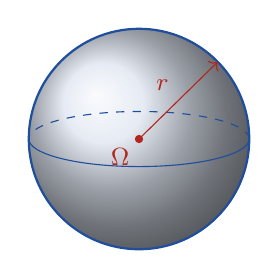
\begin{tikzpicture}[font=\small]
\shade[ball color=cDef!15] (0,0) circle (1.4); \draw[cDef,thick] (0,0) circle (1.4);
\draw[cDef,dashed] (1.4,0) arc (0:180:1.4 and 0.35); \draw[cDef] (-1.4,0) arc (180:360:1.4 and 0.35);
\fill[cThm] (0,0) circle (1.5pt) node[below left]{$\Omega$}; \draw[cThm,->] (0,0)--(1,0.98) node[midway,above left]{$r$};
\end{tikzpicture}\end{LTR}\par }{}{}
\Row{بناء المعارف}{%
\Lab{cThm}{معادلات}\par\textbf{(1)} سطح كرة مركزه $\LW{\Omega(a;b;c)}$ ونصف قطره $\LW{r}$: \par $\LW{\RR{(x-a)^2+(y-b)^2+(z-c)^2=r^2}}$.\par\textbf{(2)} أسطوانة دورانية محورها $\LW{(Oz)}$ ونصف قطرها $\LW{r}$: $\LW{\RR{x^2+y^2=r^2}}$.\par\textbf{(3)} مخروط دوراني رأسه $\LW{O}$ ومحوره $\LW{(Oz)}$ ونصف زاويته $\LW{\alpha}$: $\LW{\RR{x^2+y^2=(\tan\alpha)^2z^2}}$.}{50 د}{إكمال المربع.}
\Row{}{%
\Lab{cEx}{أمثلة محلولة}\par\textbf{(1)} $x^2+y^2+z^2-2x+4y-4=0$: $(x-1)^2-1+(y+2)^2-4+z^2-4=0$.\par\textbf{(2)} $(x-1)^2+(y+2)^2+z^2=9$: \RR{سطح} \RR{كرة} \RR{مركزه} \RR{$\Omega(1;-2;0)$} \RR{ونصف} \RR{قطره} \RR{$3$}.\par\textbf{(3)} $x^2+y^2=3z^2$: $\tan^2\alpha=3$ ، $\alpha=\dfrac\pi3$: \RR{مخروط} \RR{دوراني}.\par\textbf{(4)} $x^2+y^2+z^2=25$ و $z=3$: $x^2+y^2=16$: \RR{دائرة} \RR{مركزها} \RR{$(0;0;3)$} \RR{ونصف} \RR{قطرها} \RR{$4$}.}{}{}
\Row{}{%
\Lab{cThm!80!black}{حذار}\ نكمل المربعات قبل الحكم ؛ إذا كان الطرف الأيمن سالبًا فالمجموعة خالية. (شعبة العلوم التجريبية لا تدرس هذه المعادلات.)}{}{}
\Row{التقويم}{%
\Lab{cMeth}{تمرين تطبيقي}\par\textbf{(1)} اكتب معادلة سطح الكرة الذي مركزه $A(1;0;1)$ ويشمل $O$.\par\textbf{(2)} عيّن تقاطعه مع المستوي $z=1$.}{25 د}{تقويم فردي.}
\Row{}{%
\Lab{cEx}{حل التمرين التطبيقي}\par\textbf{(1)} $r^2=AO^2=1+0+1=2$: $\RR{(x-1)^2+y^2+(z-1)^2=2}$.\par\textbf{(2)} $z=1$: $(x-1)^2+y^2=2$: \RR{دائرة} \RR{مركزها} \RR{$A$} \RR{ونصف} \RR{قطرها} \RR{$\sqrt2$}.\par\textbf{واجب منزلي:} تمارين من باب الهندسة في الفضاء (الكرة ، الأسطوانة ، المخروط).\par\smallskip\textbf{ملاحظات حول سير الحصة:} \dotfill}{}{}
\end{Sayr}
\newpage
\ModhHead{82}{3 ع ت / 3 ر / 3 ت ر}{هندسة}{الهندسة في الفضاء}{02 سا}{التمثيل الوسيطي لمستقيم ، الوضع النسبي لمستقيمين}%
{\begin{itemize}\item الأشعة ، الارتباط الخطي.\end{itemize}}%
{\begin{itemize}\item تعيين تمثيل وسيطي لمستقيم ، ودراسة الوضع النسبي لمستقيمين.\end{itemize}}%
{المنهاج ، الكتاب المدرسي (الجزء الثاني) ، مجسمات ، برمجية Geogebra.}
\begin{Sayr}
\Row{مرحلة الانطلاق}{%
\textbf{التهيئة النفسية:} مستقيمان في الفضاء لا يتقاطعان: هل هما بالضرورة متوازيان؟}{10 د}{سؤال.}
\Row{التشخيص والاكتشاف}{%
\Lab{cEx}{نشاط رقم 04}\ $(D)$ يشمل $A(1;0;3)$ وشعاع توجيهه $\vec u(1;2;-1)$.\par\textbf{(1)} ترجم $M(x;y;z)\in(D)$ بشعاعين.\par\textbf{(2)} استنتج $x$ ، $y$ ، $z$ بدلالة وسيط $t$.}{35 د}{الحل بوسيطين.}
\Row{}{%
\Lab{cDef}{مناقشة النشاط}\par\textbf{(1)} $M\in(D)\iff\overrightarrow{AM}=t\vec u$ ($t\in\mathbb R$).\par\textbf{(2)} $\RR{x=1+t}$ ، $\RR{y=2t}$ ، $\RR{z=3-t}$.}{}{}
\Row{بناء المعارف}{%
\Lab{cThm}{خاصية}\ المستقيم الذي يشمل $\LW{A}$ وشعاع توجيهه $\LW{\vec u(a;b;c)}$: \par $\LW{\RR{x=x_A+at\ ;\ y=y_A+bt\ ;\ z=z_A+ct}}$ ($\LW{t\in\mathbb R}$).}{50 د}{جدول الحالات.}
\Row{}{%
\Lab{cMeth}{وضع مستقيمين}\par\textbf{(1)} شعاعا التوجيه مرتبطان خطيًا: \RR{متوازيان} (أو \RR{منطبقان} إذا اشتركا في نقطة).\par\textbf{(2)} غير مرتبطين: نحل الجملة بوسيطين $\LW{t}$ و $\LW{s}$: حل وحيد = \RR{متقاطعان} ، لا حل = \RR{ليسا} \RR{من} \RR{نفس} \RR{المستوي}.}{}{}
\Row{}{%
\Lab{cEx}{أمثلة محلولة}\ $(D_1)$: $(1+t;2t;3-t)$ ، $(D_2)$: $(s;-1+s;4-2s)$ ، $(D_4)$: $(2+s;2-s;2+s)$.\par\textbf{(1)} $(D_1)$ و $(D_2)$: الشعاعان $(1;2;-1)$ و $(1;1;-2)$ غير مرتبطين ؛ $1+t=s$ و $2t=-1+s$ يعطيان $t=0$ ، $s=1$.\par\textbf{(2)} $z$: $3\neq4-2=2$: \RR{ليسا} \RR{من} \RR{نفس} \RR{المستوي}.\par\textbf{(3)} $(D_1)$ و $(D_4)$: $1+t=2+s$ و $2t=2-s$: $t=1$ ، $s=0$ ؛ $z$: $2=2$ \ck: \RR{متقاطعان} \RR{في} \RR{$(2;2;2)$}.}{}{}
\Row{}{%
\Lab{cThm!80!black}{حذار}\ نستعمل وسيطين مختلفين $t$ و $s$ ، ونتحقق من المعادلة الثالثة.}{}{}
\Row{التقويم}{%
\Lab{cMeth}{تمرين تطبيقي}\par $(D_3)$: $x=2+k$ ، $y=2+2k$ ، $z=2-k$.\par\textbf{(1)} ما وضع $(D_1)$ و $(D_3)$ ؟}{25 د}{تقويم فردي.}
\Row{}{%
\Lab{cEx}{حل التمرين التطبيقي}\par\textbf{(1)} نفس شعاع التوجيه $(1;2;-1)$ ، و $(2;2;2)\in(D_1)$ (من أجل $t=1$): \RR{منطبقان}.\par\textbf{واجب منزلي:} تمارين من باب الهندسة في الفضاء.\par\smallskip\textbf{ملاحظات حول سير الحصة:} \dotfill}{}{}
\end{Sayr}
\newpage
\ModhHead{83}{3 ع ت / 3 ر / 3 ت ر}{هندسة}{الهندسة في الفضاء}{02 سا}{الجداء السلمي في الفضاء ، التعامد}%
{\begin{itemize}\item الجداء السلمي في المستوي.\end{itemize}}%
{\begin{itemize}\item حساب الجداء السلمي بالعبارة التحليلية ، وإثبات تعامد شعاعين أو مستقيمين.\end{itemize}}%
{المنهاج ، الكتاب المدرسي (الجزء الثاني) ، مجسمات ، برمجية Geogebra.}
\begin{Sayr}
\Row{مرحلة الانطلاق}{%
\textbf{التهيئة النفسية:} كيف نتحقق أن حرفين في مكعب متعامدان باستعمال الإحداثيات؟}{10 د}{سؤال.}
\Row{التشخيص والاكتشاف}{%
\Lab{cEx}{نشاط رقم 05}\par\textbf{(1)} $\vec u(x;y;z)$: احسب $\|\vec u\|^2$.\par\textbf{(2)} باستعمال \par $\vec u\cdot\vec v=\dfrac12\left(\|\vec u+\vec v\|^2-\|\vec u\|^2-\|\vec v\|^2\right)$ ، عبّر عن $\vec u\cdot\vec v$ بالمركبات.}{35 د}{التمديد من المستوي.}
\Row{}{%
\Lab{cDef}{مناقشة النشاط}\par\textbf{(1)} $\|\vec u\|^2=\RR{x^2+y^2+z^2}$.\par\textbf{(2)} بعد التبسيط: $\RR{\vec u\cdot\vec v=xx^{\prime}+yy^{\prime}+zz^{\prime}}$.}{}{}
\Row{بناء المعارف}{%
\Lab{cThm}{خاصية}\par\textbf{(1)} في معلم متعامد ومتجانس: $\LW{\RR{\vec u\cdot\vec v=xx^{\prime}+yy^{\prime}+zz^{\prime}}}$ ، و \par $\LW{\|\vec u\|=\sqrt{x^2+y^2+z^2}}$.\par\textbf{(2)} $\LW{\RR{\vec u\perp\vec v\iff\vec u\cdot\vec v=0}}$.}{50 د}{حل الجملة.}
\Row{}{%
\Lab{cMeth}{شعاع عمودي على شعاعين}\ نبحث عن $\LW{\vec n(a;b;c)\neq\vec0}$ حيث $\LW{\vec n\cdot\vec v=0}$ و $\LW{\vec n\cdot\vec w=0}$ ، ونثبت مثلًا $\LW{c=1}$.}{}{}
\Row{}{%
\Lab{cEx}{مثال محلول}\ $\vec v(-2;1;7)$ ، $\vec w(1;2;3)$ ، و $c=1$:\par\textbf{(1)} $-2a+b+7=0$ و $a+2b+3=0$: $b=2a-7$ ، ثم $5a-11=0$.\par\textbf{(2)} $a=\dfrac{11}5$ ، $b=-\dfrac{13}5$: $\RR{\vec n(11;-13;5)}$ (تحقق: $-22-13+35=0$ \ck).}{}{}
\Row{}{%
\Lab{cThm!80!black}{حذار}\ $\vec n$ معرف بتقريب عامل غير معدوم: $(11;-13;5)$ و \par $\left(\frac{11}5;-\frac{13}5;1\right)$ نفس الاتجاه.}{}{}
\Row{التقويم}{%
\Lab{cMeth}{تمرين تطبيقي}\par $A(1;1;1)$ ، $B(2;3;1)$ ، $C(3;0;1)$.\par\textbf{(1)} بيّن أن المثلث $ABC$ قائم في $A$.}{25 د}{تقويم فردي.}
\Row{}{%
\Lab{cEx}{حل التمرين التطبيقي}\par\textbf{(1)} $\overrightarrow{AB}(1;2;0)$ ، $\overrightarrow{AC}(2;-1;0)$: $\overrightarrow{AB}\cdot\overrightarrow{AC}=2-2+0=\RR{0}$: \RR{قائم} \RR{في} \RR{$A$}.\par\textbf{واجب منزلي:} تمارين من باب الجداء السلمي في الفضاء.\par\smallskip\textbf{ملاحظات حول سير الحصة:} \dotfill}{}{}
\end{Sayr}
\newpage
\ModhHead{84}{3 ع ت / 3 ر / 3 ت ر}{هندسة}{الهندسة في الفضاء}{02 سا}{معادلة مستو}%
{\begin{itemize}\item الجداء السلمي في الفضاء.\end{itemize}}%
{\begin{itemize}\item تعيين معادلة ديكارتية لمستو ، والتعرف على مستو من معادلته.\end{itemize}}%
{المنهاج ، الكتاب المدرسي (الجزء الثاني) ، مجسمات ، برمجية Geogebra.}
\begin{Sayr}
\Row{مرحلة الانطلاق}{%
\textbf{التهيئة النفسية:} ما مجموعة النقط $M$ حيث $\overrightarrow{AM}\cdot\vec n=0$ ؟}{10 د}{سؤال.}
\Row{التشخيص والاكتشاف}{%
\Lab{cEx}{نشاط رقم 06}\ $A(1;2;-1)$ و $\vec n(2;-1;3)$.\par\textbf{(1)} ترجم $\overrightarrow{AM}\cdot\vec n=0$ بدلالة $x$ ، $y$ ، $z$.\par\textbf{(2)} ما طبيعة هذه المجموعة؟}{35 د}{التمديد.}
\Row{}{%
\Lab{cDef}{مناقشة النشاط}\par\textbf{(1)} $2(x-1)-(y-2)+3(z+1)=0$: $\RR{2x-y+3z+3=0}$.\par\textbf{(2)} \RR{مستو} يشمل $A$ وعمودي على $\vec n$.}{}{}
\Row{بناء المعارف}{%
\Lab{cThm}{خاصية}\par\textbf{(1)} المستوي الذي $\LW{\vec n(a;b;c)}$ شعاع ناظمي له: $\LW{\RR{ax+by+cz+d=0}}$.\par\textbf{(2)} وعكسيًا: $\LW{ax+by+cz+d=0}$ مع $\LW{(a;b;c)\neq(0;0;0)}$ معادلة مستو ناظمه $\LW{\vec n(a;b;c)}$.}{50 د}{التحقق بالتعويض.}
\Row{}{%
\Lab{cMeth}{مستو يشمل ثلاث نقط}\par\textbf{(1)} نعين $\LW{\vec n}$ عموديًا على $\LW{\overrightarrow{AB}}$ و $\LW{\overrightarrow{AC}}$.\par\textbf{(2)} نعين $\LW{d}$ بتعويض $\LW{A}$ ، ونتحقق بـ $\LW{B}$ و $\LW{C}$.}{}{}
\Row{}{%
\Lab{cEx}{مثال محلول}\ $A(1;0;0)$ ، $B(0;2;0)$ ، $C(0;0;3)$: $\vec n(6;3;2)$.\par\textbf{(1)} $\overrightarrow{AB}(-1;2;0)\cdot\vec n=-6+6=0$ \ck ؛ \quad $\overrightarrow{AC}(-1;0;3)\cdot\vec n=-6+6=0$ \ck\par\textbf{(2)} $6\times1+d=0$: $d=-6$: $\RR{6x+3y+2z-6=0}$.}{}{}
\Row{}{%
\Lab{cThm!80!black}{حذار}\ نتحقق بتعويض النقط الثلاث في المعادلة.}{}{}
\Row{التقويم}{%
\Lab{cMeth}{تمرين تطبيقي}\par $A(1;2;0)$ ، $B(3;1;2)$.\par\textbf{(1)} اكتب معادلة المستوي الذي يشمل $O$ ويعامد $(AB)$.}{25 د}{تقويم فردي.}
\Row{}{%
\Lab{cEx}{حل التمرين التطبيقي}\par\textbf{(1)} $\vec n=\overrightarrow{AB}(2;-1;2)$ ، و $O$ يحقق $d=0$: $\RR{2x-y+2z=0}$.\par\textbf{واجب منزلي:} تمارين من باب الجداء السلمي في الفضاء.\par\smallskip\textbf{ملاحظات حول سير الحصة:} \dotfill}{}{}
\end{Sayr}
\newpage
\ModhHead{85}{3 ع ت / 3 ر / 3 ت ر}{هندسة}{الهندسة في الفضاء}{02 سا}{المسافة بين نقطة ومستو ، مجموعات نقط}%
{\begin{itemize}\item معادلة مستو ، الجداء السلمي.\end{itemize}}%
{\begin{itemize}\item حساب المسافة بين نقطة ومستو ، وتعيين مجموعات نقط.\end{itemize}}%
{المنهاج ، الكتاب المدرسي (الجزء الثاني) ، مجسمات ، برمجية Geogebra.}
\begin{Sayr}
\Row{مرحلة الانطلاق}{%
\textbf{التهيئة النفسية:} ما أقصر مسافة من نقطة إلى أرضية الغرفة؟}{10 د}{سؤال.}
\Row{التشخيص والاكتشاف}{%
\Lab{cEx}{نشاط رقم 07}\ $A(1;1;1)$ و $(P)$: $2x-y+2z-6=0$.\par\textbf{(1)} $H$ المسقط العمودي لـ $A$ على $(P)$: اكتب تمثيلًا وسيطيًا لـ $(AH)$.\par\textbf{(2)} عيّن $H$ واحسب $AH$.}{35 د}{المسقط العمودي.}
\Row{}{%
\Lab{cDef}{مناقشة النشاط}\par\textbf{(1)} $(AH)$ يوازي $\vec n(2;-1;2)$: $(1+2t;1-t;1+2t)$.\par\textbf{(2)} $2(1+2t)-(1-t)+2(1+2t)-6=0$: $9t-3=0$ ، $t=\dfrac13$: \par $\RR{H\left(\dfrac53;\dfrac23;\dfrac53\right)}$ و $AH=\sqrt{\dfrac49+\dfrac19+\dfrac49}=\RR{1}$.}{}{}
\Row{بناء المعارف}{%
\Lab{cThm}{خاصية}\ \par $\LW{\RR{d\big(A;(P)\big)=\dfrac{|ax_A+by_A+cz_A+d|}{\sqrt{a^2+b^2+c^2}}}}$.}{50 د}{الدستور.}
\Row{}{%
\Lab{cThm}{المستوي المحوري}\ مجموعة النقط $M$ حيث $MA=MB$: المستوي الذي يشمل منتصف $[AB]$ وناظمه $\overrightarrow{AB}$.}{}{}
\Row{}{%
\Lab{cEx}{أمثلة محلولة}\par\textbf{(1)} بالدستور: $d=\dfrac{|2-1+2-6|}{\sqrt{4+1+4}}=\dfrac33=\RR{1}$ (نفس نتيجة النشاط).\par\textbf{(2)} $A(1;0;0)$ ، $B(3;2;0)$: المنتصف $(2;1;0)$ ، $\vec n(2;2;0)$: $2x+2y-6=0$ ، أي $\RR{x+y-3=0}$.\par\textbf{(3)} (رياضيات وتقني رياضي) $\Omega(1;-2;0)$ ، $r=3$ و $(P)$: $2x-y+2z+5=0$: \par $d=\dfrac{|2+2+0+5|}3=3=r$: \RR{المستوي} \RR{مماس} \RR{لسطح} \RR{الكرة}.}{}{}
\Row{}{%
\Lab{cThm!80!black}{حذار}\ القيمة المطلقة في البسط ، والجذر في المقام.}{}{}
\Row{التقويم}{%
\Lab{cMeth}{تمرين تطبيقي}\par\textbf{(1)} احسب المسافة بين $O$ والمستوي $x+2y+2z-9=0$.}{25 د}{تقويم فردي.}
\Row{}{%
\Lab{cEx}{حل التمرين التطبيقي}\par\textbf{(1)} $d=\dfrac{|-9|}{\sqrt{1+4+4}}=\dfrac93=\RR{3}$.\par\textbf{واجب منزلي:} تمارين من باب الجداء السلمي في الفضاء.\par\smallskip\textbf{ملاحظات حول سير الحصة:} \dotfill}{}{}
\end{Sayr}
\newpage
\ModhHead{86}{3 ع ت / 3 ر / 3 ت ر}{هندسة}{الهندسة في الفضاء}{02 سا}{الأوضاع النسبية لمستقيم ومستو ، ولمستويين}%
{\begin{itemize}\item التمثيل الوسيطي ، معادلة مستو.\end{itemize}}%
{\begin{itemize}\item دراسة الوضع النسبي لمستقيم ومستو ، ولمستويين ، وتعيين التقاطع.\end{itemize}}%
{المنهاج ، الكتاب المدرسي (الجزء الثاني) ، مجسمات ، برمجية Geogebra.}
\begin{Sayr}
\Row{مرحلة الانطلاق}{%
\textbf{التهيئة النفسية:} مستقيم ومستو: ما الحالات الممكنة؟}{10 د}{سؤال.}
\Row{التشخيص والاكتشاف}{%
\Lab{cEx}{نشاط رقم 08}\ $(D)$: $(1+t;2t;3-t)$ و $(P)$: $x+y+z-6=0$.\par\textbf{(1)} عوّض التمثيل الوسيطي في معادلة $(P)$.\par\textbf{(2)} استنتج الوضع النسبي.}{35 د}{التعويض.}
\Row{}{%
\Lab{cDef}{مناقشة النشاط}\par\textbf{(1)} $1+t+2t+3-t-6=0$: $\RR{2t-2=0}$ ، $t=1$.\par\textbf{(2)} حل وحيد: \RR{متقاطعان} \RR{في} \RR{$(2;2;2)$}.}{}{}
\Row{بناء المعارف}{%
\Lab{cMeth}{مستقيم ومستو}\par\textbf{(1)} حل وحيد: \RR{متقاطعان} ؛ لا حل: \RR{متوازيان} \RR{تمامًا} ؛ كل $\LW{t}$ حل: \RR{المستقيم} \RR{محتوى} \RR{في} \RR{المستوي}.}{50 د}{جدول الحالات.}
\Row{}{%
\Lab{cMeth}{مستويان}\par\textbf{(1)} ناظمان مرتبطان خطيًا: \RR{متوازيان} (أو منطبقان).\par\textbf{(2)} وإلا: \RR{يتقاطعان} \RR{وفق} \RR{مستقيم} نعين تمثيلًا وسيطيًا له.}{}{}
\Row{}{%
\Lab{cEx}{أمثلة محلولة}\par\textbf{(1)} $x+y+z=3$ و $x-y+z=1$: بالطرح $2y=2$ ، $y=1$ ، و $x+z=2$.\par\textbf{(2)} نضع $x=t$: \RR{التقاطع} \RR{$(t;1;2-t)$} ، مستقيم يشمل $(0;1;2)$ وشعاعه $(1;0;-1)$.\par\textbf{(3)} $2x-y+z=1$ و $-4x+2y-2z=3$: الناظمان مرتبطان ($-2$) والمعادلتان غير متكافئتين: \RR{متوازيان} \RR{تمامًا}.}{}{}
\Row{}{%
\Lab{cThm!80!black}{حذار}\ نتحقق من نقطة التقاطع في كل المعادلات.}{}{}
\Row{التقويم}{%
\Lab{cMeth}{تمرين تطبيقي}\par $(D)$: $x=2t$ ، $y=1-t$ ، $z=t$ و $(P)$: $x+y-z+1=0$.\par\textbf{(1)} ما وضع $(D)$ و $(P)$ ؟}{25 د}{تقويم فردي.}
\Row{}{%
\Lab{cEx}{حل التمرين التطبيقي}\par\textbf{(1)} $2t+1-t-t+1=2\neq0$: لا حل: \RR{$(D)$} \RR{يوازي} \RR{$(P)$} \RR{تمامًا}.\par\textbf{واجب منزلي:} تمارين من باب الهندسة في الفضاء.\par\smallskip\textbf{ملاحظات حول سير الحصة:} \dotfill}{}{}
\end{Sayr}
\newpage
\ModhHead{87}{3 ع ت / 3 ر / 3 ت ر}{هندسة}{الهندسة في الفضاء}{02 سا}{تقاطع ثلاثة مستويات ، الانتقال بين التمثيلات}%
{\begin{itemize}\item معادلة مستو ، التمثيل الوسيطي ، الجمل الخطية.\end{itemize}}%
{\begin{itemize}\item تعيين تقاطع ثلاثة مستويات ، والانتقال من جملة معادلتين لمستقيم إلى تمثيل وسيطي والعكس.\end{itemize}}%
{المنهاج ، الكتاب المدرسي (الجزء الثاني) ، مجسمات ، برمجية Geogebra.}
\begin{Sayr}
\Row{مرحلة الانطلاق}{%
\textbf{التهيئة النفسية:} ثلاثة جدران في زاوية الغرفة: في كم نقطة تتقاطع؟}{10 د}{سؤال.}
\Row{التشخيص والاكتشاف}{%
\Lab{cEx}{نشاط رقم 09}\ $(P_1)$: $x+y+z=6$ ، $(P_2)$: $x-y+z=2$ ، $(P_3)$: $x+y-z=0$.\par\textbf{(1)} احسب $(P_1)-(P_2)$ و $(P_1)-(P_3)$.\par\textbf{(2)} استنتج التقاطع.}{35 د}{طرق الحل.}
\Row{}{%
\Lab{cDef}{مناقشة النشاط}\par\textbf{(1)} $2y=4$ ، $\RR{y=2}$ ؛ \quad $2z=6$ ، $\RR{z=3}$.\par\textbf{(2)} $x=6-2-3=\RR{1}$: \RR{نقطة} \RR{واحدة} \RR{$(1;2;3)$}.}{}{}
\Row{بناء المعارف}{%
\Lab{cMeth}{طريقة}\par\textbf{(1)} نحل الجملة بالتعويض أو بالجمع.\par\textbf{(2)} حل وحيد: \RR{نقطة} ؛ عدد لا نهائي بوسيط: \RR{مستقيم} ؛ لا حل: \RR{لا} \RR{نقطة} \RR{مشتركة}.}{50 د}{التفسير الهندسي.}
\Row{}{%
\Lab{cMeth}{من جملة إلى تمثيل وسيطي}\ نضع أحد المجاهيل وسيطًا $\LW{t}$ ونعبر عن الآخرين بدلالته ؛ والعكس: نحذف $\LW{t}$ بين المعادلات.}{}{}
\Row{}{%
\Lab{cEx}{أمثلة محلولة}\par\textbf{(1)} $x+y+z=3$ ، $x-y+z=1$ ، $2x+2z=4$: الثالثة مجموع الأوليين: \RR{مستقيم} \RR{$(t;1;2-t)$}.\par\textbf{(2)} $x=1+t$ ، $y=2t$ ، $z=3-t$: $t=x-1$ ، إذن $\RR{y=2x-2}$ و $\RR{z=4-x}$ (جملة معادلتين).}{}{}
\Row{}{%
\Lab{cThm!80!black}{حذار}\ نتحقق من الحل في المعادلات الثلاث.}{}{}
\Row{التقويم}{%
\Lab{cMeth}{تمرين تطبيقي}\par\textbf{(1)} عيّن تقاطع المستويات $x+y=3$ ، $y+z=5$ ، $x+z=4$.}{25 د}{تقويم فردي.}
\Row{}{%
\Lab{cEx}{حل التمرين التطبيقي}\par\textbf{(1)} بالجمع: $2(x+y+z)=12$ ، $x+y+z=6$.\par\textbf{(2)} $z=6-3=\RR{3}$ ، $x=6-5=\RR{1}$ ، $y=6-4=\RR{2}$: \RR{النقطة} \RR{$(1;2;3)$}.\par\textbf{واجب منزلي:} تمارين من باب الهندسة في الفضاء.\par\smallskip\textbf{ملاحظات حول سير الحصة:} \dotfill}{}{}
\end{Sayr}
\newpage
\ModhHead{88}{3 ع ت / 3 ر / 3 ت ر}{هندسة}{الهندسة في الفضاء}{02 سا}{حل مسائل في الهندسة الفضائية}%
{\begin{itemize}\item معادلة مستو ، المسافة بين نقطة ومستو ، الحجوم.\end{itemize}}%
{\begin{itemize}\item توظيف المكتسبات لحل مسائل: حجوم ، مسافات ، مساحات.\end{itemize}}%
{المنهاج ، الكتاب المدرسي (الجزء الثاني) ، مجسمات ، برمجية Geogebra.}
\begin{Sayr}
\Row{مرحلة الانطلاق}{%
\textbf{التهيئة النفسية:} كيف نحسب مساحة مثلث في الفضاء دون حساب ارتفاعه مباشرة؟}{10 د}{سؤال.}
\Row{التشخيص والاكتشاف}{%
\Lab{cEx}{نشاط رقم 10}\ رباعي الوجوه $OABC$ مع $A(1;0;0)$ ، $B(0;2;0)$ ، $C(0;0;3)$.\par\smallskip\begin{LTR}\centering 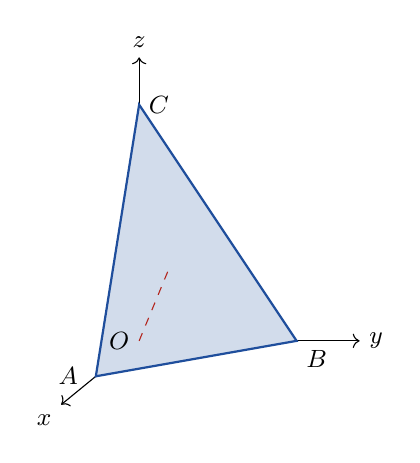
\begin{tikzpicture}[x={(-0.55cm,-0.45cm)},y={(1cm,0cm)},z={(0cm,1cm)},font=\small]
\draw[->] (0,0,0)--(1.8,0,0) node[below left]{$x$}; \draw[->] (0,0,0)--(0,2.8,0) node[right]{$y$}; \draw[->] (0,0,0)--(0,0,3.6) node[above]{$z$};
\fill[cDef!20] (1,0,0)--(0,2,0)--(0,0,3)--cycle; \draw[cDef,thick] (1,0,0)--(0,2,0)--(0,0,3)--cycle;
\draw[cThm,dashed] (0,0,0)--(0.4,0.6,1.1);
\node[left=3pt] at (1,0,0){$A$}; \node[below right] at (0,2,0){$B$}; \node[right] at (0,0,3){$C$}; \node[left] at (0,0,0){$O$};
\end{tikzpicture}\end{LTR}\par \par\textbf{(1)} احسب حجمه باختيار القاعدة $OAB$.\par\textbf{(2)} اكتب معادلة $(ABC)$ واحسب $d\big(O;(ABC)\big)$.\par\textbf{(3)} استنتج مساحة المثلث $ABC$.}{35 د}{رسم بالمنظور.}
\Row{}{%
\Lab{cDef}{مناقشة النشاط}\par\textbf{(1)} $\mathcal A_{OAB}=\dfrac{1\times2}2=1$ والارتفاع $OC=3$: $V=\dfrac13\times1\times3=\RR{1}$ u.v.\par\textbf{(2)} $(ABC)$: $6x+3y+2z-6=0$ ؛ $d=\dfrac{|-6|}{\sqrt{36+9+4}}=\RR{\dfrac67}$.\par\textbf{(3)} $V=\dfrac13\times\mathcal A_{ABC}\times\dfrac67=1$: $\mathcal A_{ABC}=\RR{\dfrac72}$ u.a.}{}{}
\Row{بناء المعارف}{%
\Lab{cMeth}{طريقة}\par\textbf{(1)} نحسب نفس الحجم بقاعدتين مختلفتين لاستنتاج مسافة أو مساحة.\par\textbf{(2)} $\LW{\RR{V=\dfrac13\times\mathcal A\times h}}$ لرباعي الوجوه.}{50 د}{طريقتان لنفس الحجم.}
\Row{}{%
\Lab{cEx}{مثال محلول}\ $A(2;0;0)$ ، $B(0;2;0)$ ، $C(0;0;2)$:\par\textbf{(1)} $(ABC)$: $x+y+z-2=0$ ؛ $V=\dfrac13\times2\times2=\dfrac43$.\par\textbf{(2)} $d=\dfrac2{\sqrt3}$: $\mathcal A_{ABC}=\dfrac{3V}d=\dfrac{4}{2/\sqrt3}=\RR{2\sqrt3}$ u.a.}{}{}
\Row{}{%
\Lab{cThm!80!black}{حذار}\ وحدات المساحة (u.a) والحجم (u.v).}{}{}
\Row{التقويم}{%
\Lab{cMeth}{تمرين تطبيقي}\par\textbf{(1)} احسب المسافة بين $O$ والمستوي $(ABC)$ حيث $A(2;0;0)$ ، $B(0;2;0)$ ، $C(0;0;2)$.}{25 د}{نهاية المحور والسنة: مراجعة البكالوريا.}
\Row{}{%
\Lab{cEx}{حل التمرين التطبيقي}\par\textbf{(1)} $(ABC)$: $x+y+z-2=0$: $d=\dfrac2{\sqrt3}=\RR{\dfrac{2\sqrt3}3}$.\par\textbf{واجب منزلي:} مسائل من باب الهندسة في الفضاء.\par\smallskip\textbf{ملاحظات حول سير الحصة:} \dotfill}{}{}
\end{Sayr}
\end{document}
